% Interaction overview for the Budget-Aware Draft Controller.
%
% This figure deliberately uses the compact overview grammar of the two
% reference papers: one dominant execution path, one clearly named system
% boundary, and only the feedback needed to explain the interaction.  It is
% not a duration-proportional timeline and introduces no notation before the
% model and pacing subsections define it.
%
% The top row is framework execution owned outside the controller.  Parallel
% captures create Draft tasks, but those tasks serialize in capture order on
% one Draft worker.  The lower shell contains only controller-owned state and
% decisions.  Pacing points upstream to the next application-facing release;
% admission points locally to optional nodes in the active Draft Sequence.
%
% Drawn at final size (natural width about 17.2 cm).  Keep explicit line breaks
% and coordinates: the paper preamble intentionally loads only the basic TikZ
% libraries used elsewhere in the manuscript.
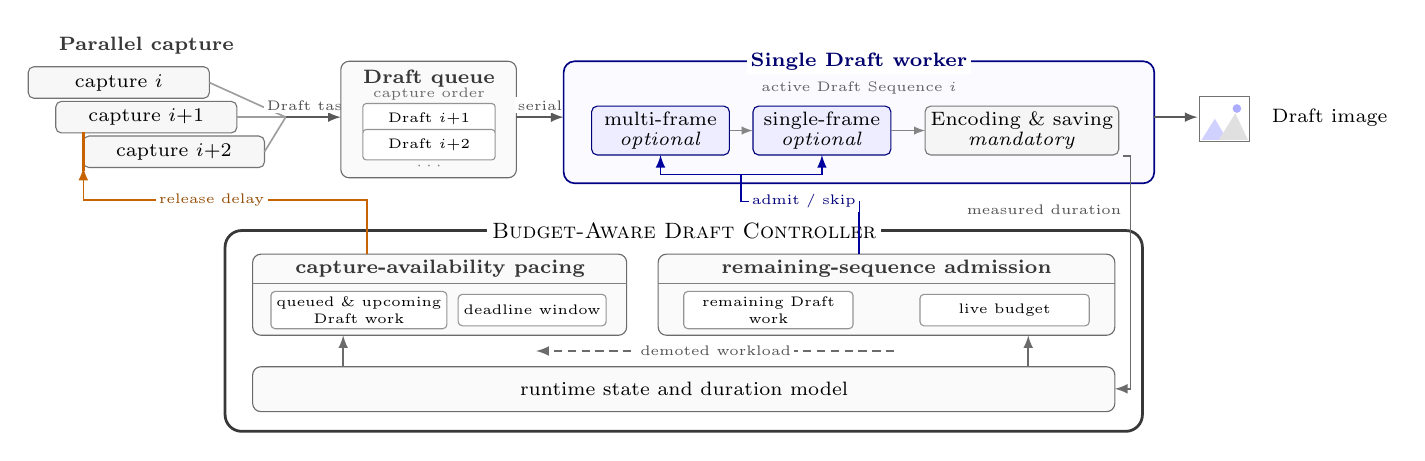
\begin{tikzpicture}[
  x=1cm, y=1cm, >=latex, font=\scriptsize,
  shell/.style={draw=black!78, line width=1pt, rounded corners=6pt},
  stage/.style={draw=black!58, fill=black!2, rounded corners=3pt},
  cell/.style={draw=black!42, fill=white, rounded corners=1.5pt,
    align=center, inner sep=2pt, font=\tiny, minimum height=0.40cm},
  capture/.style={draw=black!55, fill=black!3, rounded corners=2pt},
  queue/.style={draw=black!58, fill=black!2, rounded corners=3pt},
  queuecard/.style={draw=black!42, fill=white, rounded corners=1.2pt,
    align=center, font=\tiny, minimum height=0.25cm},
  worker/.style={draw=blue!52!black, fill=blue!2, rounded corners=4pt,
    semithick},
  optional/.style={draw=blue!48!black, fill=blue!7, rounded corners=2pt,
    align=center, inner sep=2pt, minimum height=0.62cm},
  mandatory/.style={draw=black!52, fill=black!4, rounded corners=2pt,
    align=center, inner sep=2pt, minimum height=0.62cm},
  flow/.style={->, semithick, black!65},
  nodeflow/.style={->, thin, black!48},
  merge/.style={semithick, black!38},
  pace/.style={->, semithick, orange!78!black},
  admit/.style={->, semithick, blue!62!black},
  state/.style={->, semithick, densely dashed, black!58},
  feedback/.style={->, semithick, black!58},
  heading/.style={font=\scriptsize\bfseries, text=black!78},
  lab/.style={font=\tiny, text=black!68, fill=white, inner sep=1.2pt},
  accentlab/.style={font=\tiny, fill=white, inner sep=1.2pt}
]

  % ==================================================== framework execution
  % Three offset request cards show concurrency without pretending that their
  % horizontal lengths are measured durations.
  \node[heading] at (1.65,5.10) {Parallel capture};
  \draw[capture] (0.15,4.43) rectangle (2.45,4.83);
  \node at (1.30,4.63) {capture $i$};
  \draw[capture] (0.50,3.99) rectangle (2.80,4.39);
  \node at (1.65,4.19) {capture $i{+}1$};
  \draw[capture] (0.85,3.55) rectangle (3.15,3.95);
  \node at (2.00,3.75) {capture $i{+}2$};

  % The pacing arrow terminates at the start of the newest capture card.  The
  % small gate marks release of the callback, not Draft-task admission.
  \draw[orange!78!black, line width=1.2pt] (0.85,3.50) -- (0.85,4.00);

  % Capture requests yield Draft tasks, which merge into one ordered queue.
  \draw[merge] (2.45,4.63) -- (3.42,4.19);
  \draw[merge] (2.80,4.19) -- (3.42,4.19);
  \draw[merge] (3.15,3.75) -- (3.42,4.19);
  \draw[flow] (3.42,4.19) -- (4.12,4.19);
  \node[lab, anchor=south] at (3.77,4.23) {Draft tasks};

  % A visible FIFO makes the cross-shot bottleneck explicit.
  \draw[queue] (4.12,3.42) rectangle (6.35,4.90);
  \node[heading] at (5.24,4.68) {Draft queue};
  \node[font=\tiny, text=black!58] at (5.24,4.48) {capture order};
  \node[queuecard, minimum width=1.68cm] at (5.24,4.17) {Draft $i{+}1$};
  \node[queuecard, minimum width=1.68cm] at (5.24,3.84) {Draft $i{+}2$};
  \node[font=\tiny, text=black!52] at (5.24,3.57) {$\cdots$};

  \draw[flow] (6.35,4.19) -- (6.95,4.19);
  \node[lab, anchor=south] at (6.65,4.23) {serial};

  % Only the active Draft is expanded.  Optional work is visually distinct
  % from the mandatory tail but is not pre-labelled as admitted or skipped.
  \draw[worker] (6.95,3.35) rectangle (14.45,4.90);
  \node[fill=white, inner sep=1.4pt, font=\scriptsize\bfseries,
    text=blue!43!black] at (10.70,4.90) {Single Draft worker};
  \node[font=\tiny, text=black!62] at (10.70,4.56)
    {active Draft Sequence $i$};
  \node[optional, minimum width=1.75cm] at (8.18,4.02)
    {multi-frame\\[-1pt]\textit{optional}};
  \node[optional, minimum width=1.75cm] at (10.23,4.02)
    {single-frame\\[-1pt]\textit{optional}};
  \node[mandatory, minimum width=2.45cm] at (12.77,4.02)
    {Encoding \& saving\\[-1pt]\textit{mandatory}};
  \draw[nodeflow] (9.06,4.02) -- (9.35,4.02);
  \draw[nodeflow] (11.11,4.02) -- (11.54,4.02);

  % Draft publication remains outside the controller boundary.
  \draw[flow] (14.45,4.19) -- (15.00,4.19);
  \fill[white] (15.03,3.88) rectangle (15.66,4.45);
  \fill[blue!18] (15.05,3.90) -- (15.22,4.17) -- (15.38,3.90) -- cycle;
  \fill[black!12] (15.27,3.90) -- (15.48,4.24) -- (15.64,3.90) -- cycle;
  \fill[blue!32] (15.50,4.30) circle (0.055);
  \draw[black!55] (15.03,3.88) rectangle (15.66,4.45);
  \node[anchor=west] at (15.82,4.19) {Draft image};

  % =============================================== controller-owned boundary
  \draw[shell] (2.65,0.20) rectangle (14.30,2.75);
  \node[fill=white, inner sep=1.8pt, font=\footnotesize\scshape]
    at (8.48,2.75) {Budget-Aware Draft Controller};

  % Pacing controls a future arrival.
  \draw[stage] (3.00,1.42) rectangle (7.75,2.45);
  \draw[black!50] (3.00,2.08) -- (7.75,2.08);
  \node[heading] at (5.38,2.27) {capture-availability pacing};
  \node[cell, minimum width=2.20cm] at (4.35,1.74)
    {queued \& upcoming\\Draft work};
  \node[cell, minimum width=1.70cm] at (6.55,1.74)
    {deadline window};

  % Admission controls optional work in the Draft that owns the worker.
  \draw[stage] (8.15,1.42) rectangle (13.95,2.45);
  \draw[black!50] (8.15,2.08) -- (13.95,2.08);
  \node[heading] at (11.05,2.27) {remaining-sequence admission};
  \node[cell, minimum width=2.15cm] at (9.55,1.74)
    {remaining Draft\\work};
  \node[cell, minimum width=2.15cm] at (12.55,1.74)
    {live budget};

  % Both actuators read the same learned and queue-local state.
  \draw[stage] (3.00,0.45) rectangle (13.95,1.02);
  \node at (8.48,0.74) {runtime state and duration model};
  \draw[feedback] (4.15,1.02) -- (4.15,1.42);
  \draw[feedback] (12.85,1.02) -- (12.85,1.42);

  % Admission changes the workload shape seen by later pacing decisions.  The
  % reverse direction is deliberately absent: pacing affects later admission
  % only through the real arrival/queue/budget path drawn above.
  \draw[state] (11.15,1.22) -- (6.60,1.22);
  \node[lab] at (8.88,1.22) {demoted workload};

  % Pacing's sole backward arrow targets the next callback release.
  \draw[pace] (4.45,2.45) -- (4.45,3.14) -- (0.85,3.14) -- (0.85,3.55);
  \node[accentlab, text=orange!58!black] at (2.48,3.14)
    {release delay};

  % Admission branches only to optional nodes of the active sequence.
  \draw[admit, -] (10.70,2.45) -- (10.70,3.12) -- (9.20,3.12)
    -- (9.20,3.46);
  \draw[admit] (9.20,3.46) -- (8.18,3.46) -- (8.18,3.71);
  \draw[admit] (9.20,3.46) -- (10.23,3.46) -- (10.23,3.71);
  \node[accentlab, text=blue!48!black] at (10.00,3.12)
    {admit / skip};

  % Learning occurs only when the Draft has completed.
  \draw[feedback] (14.05,3.70) -- (14.15,3.70) -- (14.15,0.74)
    -- (13.95,0.74);
  \node[lab, anchor=east] at (14.08,3.02) {measured duration};

\end{tikzpicture}
